\documentclass[12pt]{article}

\usepackage[english]{babel}

% Math/Greek packages
\usepackage{amssymb,amsmath,amsthm, mathtools} 
\usepackage{algorithm, algorithmic}
\usepackage{upgreek, siunitx}

% Graphics/Presentation packages
\usepackage{geometry, graphicx}
\usepackage{tabulary, enumitem, array}
\usepackage{xparse,mleftright,tikz}
\usepackage{physics}

% Misc packages
\usepackage{fancyhdr}


\usepackage[export]{adjustbox}

\usepackage{esint}

\sisetup{locale=US,group-separator = {,}}
\usepackage[colorlinks=true, allcolors=blue]{hyperref}


% General macro declarations


\makeatletter
\let\oldabs\abs
\def\abs{\@ifstar{\oldabs}{\oldabs*}}
%
\let\oldnorm\norm
\def\norm{\@ifstar{\oldnorm}{\oldnorm*}}
\makeatother

\begin{document}

\title{PHSX 425: HW11}
\author{William Jardee}
\maketitle

\noindent
\emph{In class, we solved the problem of relfection and refraction at oblique incidence to an interface between linear media, for the case of polarization in the plane of incidence.}
\section*{Question 1}
\emph{Derive $E_{0R}$ and $E_{0T}$ for the case of polarization perpendicular to the plane of incidence. Write your answer in terms of $E_{0I}$, $\alpha$, and $\beta$.}

\begin{equation}
	\tag{9.101 i}
	\varepsilon_1(\vb{E}_{0I} + \vb{E}_{0R})_z = \varepsilon_2 (\vb{E}_{0T})_z 
	\label{eq:9.101i}
\end{equation}
\begin{equation}
	\tag{9.101 ii}
	(\vb{B}_{0I} + \vb{B}_{0R})_z  = (\vb{B}_{0T})_z
	\label{eq:9.101ii}
\end{equation}
\begin{equation}
	\tag{9.101 iii}
	(\vb{E}_{0I} + \vb{E}_{0R})_{x,y} = (\vb{E}_{0T})_{x,y}
	\label{eq:9.101iii}
\end{equation}
\begin{equation}
	\tag{9.101 iv}
	\frac{1}{\mu_1}(\vb{B}_{0I} + \vb{B}_{0R})_{x,y} = \frac{1}{\mu_2}(\vb{B}_{0T})_{x,y}
	\label{eq:9.101iv}
\end{equation}

If we take the convention that is used in Griffiths, then the plane of incidence is in the xz-plane, and so the polarization of our EM wave will be perpendicular to this plane. So, the $\vb{E}$ doesn't have any components in the z-direction. So, equation \ref{eq:9.101i} becomes: $0=0$, and equation \ref{eq:9.101iii} becomes
\begin{equation}
	\vb{E}_{0I} + \vb{E}_{0R} = \vb{E}_{0T}
	\label{a}
\end{equation}

To tackle the other two equation we have to recognize that $\frac{1}{v}(\vb{k} \times \vb{E}) = \vb{B}$. Equation \ref{eq:9.101ii} becomes:
\[(\vb{B}_{0I} + \vb{B}_{0R})_z  = (\vb{B}_{0T})_z\]
\[\Big( \frac{1}{v_1}\vb{E}_{0I} + \frac{1}{v_1}\vb{0R} \Big)_z = \Big(\frac{1}{v_2}\vb{E}_{0T}\Big)_z\]
\[E_{0I}\sin(\theta_I) + E_{0R} \sin(\theta_R) = \frac{v_1}{v_2}E_{0T}\sin(\theta_T)\]
\begin{equation}
	E_{0I} + E_{0R} = \frac{v_1}{v_2}\frac{\sin(\theta_T)}{\sin(\theta_R)} E_{0T}
	\label{b}
\end{equation}

Using a similar route, equation \ref{eq:9.101iv} becomes
\[\frac{1}{\mu_1}(\vb{B}_{0I} + \vb{B}_{0R})_{x,y} = \frac{1}{\mu_2}(\vb{B}_{0T})_{x,y}\]
\[\frac{1}{\mu_1}(B_{0I}(-\cos(\theta_I) + B_{0R}\cos(\theta_R)) = \frac{1}{\mu_2}(B_{0T}(-\cos(\theta_T))\]
\[\frac{1}{\mu_1}\frac{1}{v_1}\cos(\theta_I)(-E_{0I} + E_{0R}) = -\frac{1}{\mu_2}\frac{1}{v_2}E_{0T}\cos(\theta_T)\]
\begin{equation}
	-E_{0I}+ E_{0R} = -\frac{\mu_1 v_1}{\mu_2 v_2}\frac{\cos(\theta_R)}{\theta_I} E_{0T}
	\label{c}
\end{equation}

Using $\alpha$ and $\beta$ to simplify the expressions, such that they are equation to:
\[\alpha = \frac{\cos(\theta_T)}{\cos(\theta_R)} \qquad \beta = \frac{\mu_1 v_1}{\mu_2 v_2}\]

adding together (\ref{b}) and (\ref{c})
\[2E_{0I} = (1+ \alpha \beta)E_{0T}\]
\[\boxed{E_{0T} = \frac{2}{1+\alpha \beta} E_{0I}}\]

plugging this into (\ref{a})
\[E_{0I} + E_{0R} = \frac{2}{1+\alpha \beta} E_0I\]
\[\boxed{E_{0R} = \frac{2-1-\alpha \beta}{1 + \alpha \beta} E_{0I} = \frac{1 - \alpha \beta}{1+ \alpha \beta} E_{0I}}\]

\section*{Question 2}
\emph{Also derive the reflection and transmission coefficients. Show that they sum to unity.}
We know that $I = \frac{1}{2}v \varepsilon E^2$, so for the transmission:\footnote{I take for granted the term $\cos(\theta_T)/\cos(\theta_R)$ because it is explained in Griffiths. The basis of which is about the fact that the conservation of energy into the interface is dependent of the average rate the wave front hits the interface - which is at an angle. }

\[T = \frac{I_T}{I_I} = \frac{v_2 \varepsilon_2}{v_1 \varepsilon_1} \frac{\cos(\theta_T)}{\cos(\theta_R)}\Big(\frac{E_T^2}{E_I^2}\Big)\]
\[\boxed{T = \beta \alpha \Big( \frac{2}{1 + \alpha \beta}\Big)^2}\]

And for reflection:
\[R = \frac{I_R}{I_I} = \frac{v_1 \varepsilon_1}{v_1 \varepsilon_1}\frac{\cos(\theta_R)}{\cos(\theta_T)}\Big(\frac{E_R^2}{E_T^2}\Big)\]
\[\boxed{R = \Big( \frac{1 - \alpha \beta}{1+ \alpha \beta}\Big)^2}\]

Checking that these sum to 1:
\[T+R = \beta \alpha \Big(\frac{2}{1+ \alpha \beta}\Big)^2 + \Big( \frac{1 - \alpha \beta}{1 + \alpha \beta}\Big)^2\]
\[= \frac{4 \alpha \beta + 1 - 2 \alpha \beta + (\alpha \beta)^2}{(1 + \alpha \beta)^2}\]
\[= \frac{1 + 2 \alpha \beta + (\alpha \beta)^2}{(1+ \alpha \beta)^2}\]
\[= \frac{(1+ \alpha \beta)^2}{(1 + \alpha \beta)^2} = 1 \, \checkmark\]



\section*{Question 3}
\emph{Using the values $n_1 = 1$, $n_2 = 1.5$, with $\mu_1 = \mu_2 = \mu_0$, plot $E_{0R}/E_{0T}$ and $E_{0T}/E_{0I}$ as a function of the incidence angle, $\theta_I$.}
\begin{figure}[ht]
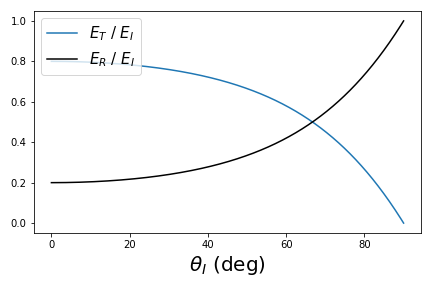
\includegraphics[scale=1]{./phsx425_hw11_3.png}
\caption{graph for \textbf{Question 3}}
\end{figure}

\section*{Question 4}
\emph{Also plot the reflection and transmission coefficients as a function of $\theta_I$.}
\begin{figure}[ht]
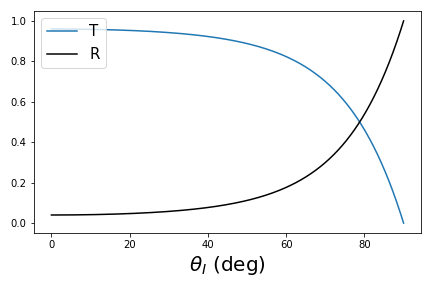
\includegraphics[scale=1]{./phsx425_hw11_4.png}
\caption{graph for \textbf{Question 4}}
\end{figure}

\clearpage 
\noindent
The code used to plot both graphs:\bigskip

\noindent
import astropy.units as u\\
import numpy as np\\
from astropy.constants import mu0\\
import matplotlib.pyplot as plt\bigskip

\noindent
n1 = 1\\
n2 = 1.5\\
mu1 = mu0\\
mu2 = mu0\\
beta = (mu1*n2)/(mu2*n1)\\
t\_T = lambda t\_I: (np.arcsin(n1 * np.sin(t\_I)/n2)).to(u.deg)\\
alpha = lambda t\_I: np.cos(t\_T(t\_I))/np.cos(t\_I)\\
E\_T = lambda t\_I : abs(2./(1+alpha(t\_I)*beta))\\
E\_R = lambda t\_I: abs((1-alpha(t\_I)*beta)/(1+alpha(t\_I)*beta))\bigskip

\noindent
T = lambda t\_I: beta*alpha(t\_I)*(E\_T(t\_I))**2\\
R = lambda t\_I: (E\_R(t\_I))**2\bigskip

\noindent
x = np.linspace(0, 90, 1000)*u.deg\\
plt.plot(x, E\_T(x), label=r'$E_T$ / $E_I$')\\
plt.plot(x, E\_R(x), color='black', label=r'$E_R$ / $E_I$')\\
plt.xlabel(r"$\theta_I$ (deg)", fontsize=20)\\
plt.legend(fontsize=15, loc='upper left')\\
plt.tight\_layout()\\
plt.savefig('phsx425\_hw11\_3')\\
plt.show()\bigskip

\noindent
x = np.linspace(0, 90, 1000)*u.deg\\
plt.plot(x, T(x), label=r'T')\\
plt.plot(x, R(x), color='black', label=r'R')\\
plt.xlabel(r"$\theta_I$ (deg)", fontsize=20)\\
plt.legend(fontsize=15, loc='upper left')\\
plt.tight\_layout()\\
plt.savefig('phsx425\_hw11\_4')\\
plt.show()\\

\end{document}